\chapter{Конструкторский раздел}

На рисунках \ref{img:aes} представлены схемы алгоритма AES, раунда AES.

\includeimage
{aes} % Имя файла без расширения (файл должен быть расположен в директории inc/img/)
{f} % Обтекание (без обтекания)
{ht!} % Положение рисунка (см. figure из пакета float)
{0.6\textwidth} % Ширина рисунка
{Схема шифровального алгоритма AES} % Подпись рисунка

%\begin{figure}[ht!]
%	\centering
%	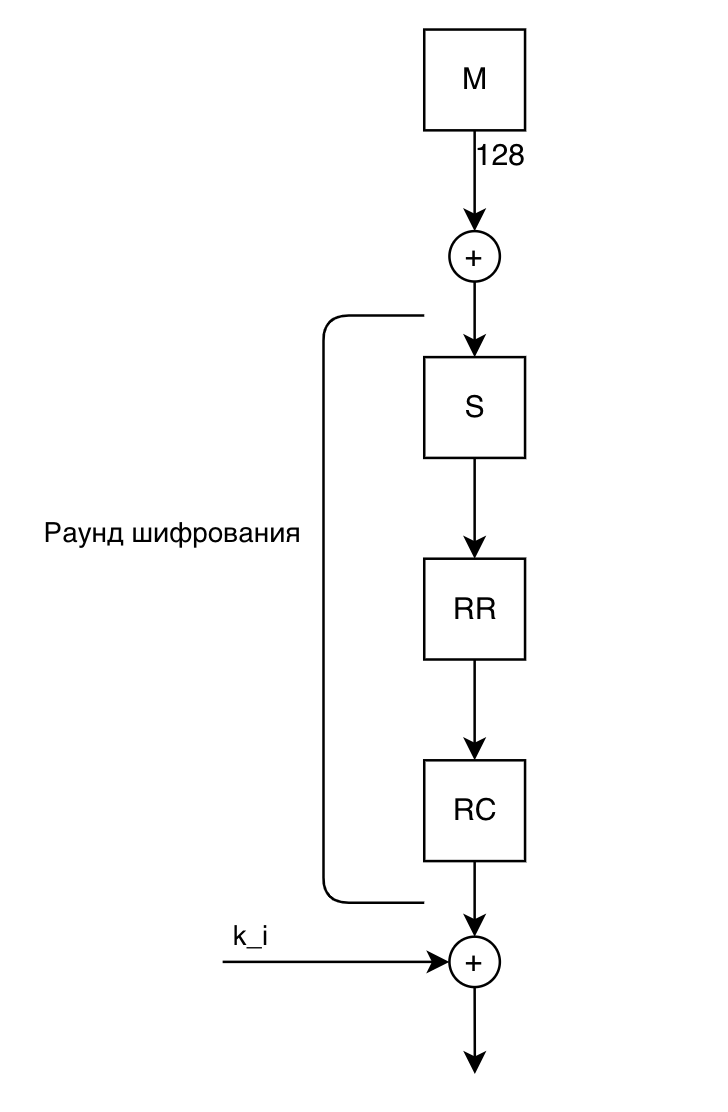
\includegraphics[width=0.6\linewidth]{img/aes.png}
%	\caption{Схема шифровального алгоритма AES}
%	\label{img:aes}
%\end{figure}

\section*{Вывод}

В этом разделе была представлена схема алгоритма шифрования AES.




